\chapter{Kết quả ứng dụng}
\label{chap:results}

\section{Đặc tả yêu cầu phần mềm}

\subsection{Mô tả tổng quan}

PERFIN là nguyên mẫu ứng dụng di động phục vụ nhập, chuẩn hóa, quản lý và phân tích dữ liệu tài chính cá nhân. Giao diện chat và media là cổng thu nhận bổ sung cho biểu mẫu. Mọi phép tính tài chính, kiểm tra ràng buộc và thay đổi dữ liệu do backend thực hiện; LLM, OCR và STT không truy cập trực tiếp PostgreSQL và không được xem là nguồn số liệu chuẩn. Cách mã hóa FR/NFR và truy vết sang ca kiểm thử vận dụng hướng dẫn kỹ nghệ yêu cầu của ISO/IEC/IEEE~29148:2018 \cite{iso29148}.

\begin{table}[H]
  \centering
  \caption{Bối cảnh vận hành và ràng buộc của sản phẩm}
  \label{tab:product-overview}
  \begin{tabularx}{\textwidth}{@{}L{3.5cm}Y@{}}
    \toprule
    \textbf{Hạng mục} & \textbf{Mô tả} \\
    \midrule
    Người dùng & Một người dùng phổ thông cần ghi chép và hiểu dữ liệu tài chính; không yêu cầu kiến thức thống kê. \\
    Môi trường & React Native/Expo trên mobile hoặc web; Express API; PostgreSQL; Redis và worker là thành phần tùy cấu hình. \\
    Dữ liệu chuẩn & PostgreSQL lưu dữ liệu nghiệp vụ; Redis chỉ lưu pending, clarification, cache và queue có TTL. \\
    Ràng buộc & Phiên bản demo dùng \code{default_user}, chưa có authentication/authorization production; tiền mặc định là VND và chưa có quy đổi ngoại tệ. \\
    Phụ thuộc & Gemini là provider ngôn ngữ bên ngoài; PaddleOCR và PhoWhisper chạy cục bộ trên backend. Media cục bộ lỗi thì báo lỗi thật, không tạo dữ liệu giả. \\
    Giả định & Người dùng kiểm tra bản xem trước; gợi ý không thay thế tư vấn tài chính chuyên nghiệp. \\
    \bottomrule
  \end{tabularx}
\end{table}

\begin{table}[H]
  \centering
  \caption{Tác nhân và mối quan tâm}
  \label{tab:actors}
  \begin{tabularx}{\textwidth}{@{}L{3.2cm}Y Y@{}}
    \toprule
    \textbf{Tác nhân} & \textbf{Vai trò} & \textbf{Mối quan tâm/giới hạn} \\
    \midrule
    Người dùng & Nhập, sửa, xác nhận, quản lý và xem báo cáo. & Dữ liệu suy ra từ ngôn ngữ/media phải được kiểm tra trước khi lưu. \\
    Adapter AI ngoài/cục bộ & Gemini trả typed draft hoặc narration; runtime media cục bộ trả OCR text hoặc transcript. & Không adapter nào được gọi nghiệp vụ hay ghi database; text trích xuất vẫn không đáng tin tuyệt đối. \\
    Worker nền & Chạy lịch nhắc, phân tích và dọn tệp. & Job phải có user scope, retry và chống hiệu ứng lặp. \\
    Quản trị viên phát triển & Cấu hình môi trường, migration và provider. & Không phải tác nhân nghiệp vụ của ứng dụng. \\
    \bottomrule
  \end{tabularx}
\end{table}

Các quy tắc dùng chung là: số tiền nghiệp vụ phải hữu hạn và đúng miền; ngày giao dịch không ở tương lai; ví/danh mục phải thuộc hồ sơ hiện tại; số dư ví được phép âm; thao tác khởi tạo từ chat/media phải qua preview và xác nhận; cập nhật nhiều bản ghi phải nguyên tử; báo cáo mặc định loại giao dịch đã soft delete; thiếu dữ liệu phải trả cảnh báo hoặc \code{null} thay vì suy diễn.

\subsection{Yêu cầu chức năng}

\widereportfigure{14-usecase-overview.pdf}{Sơ đồ use case tổng thể của PERFIN. Chi tiết từng chức năng được mô tả bằng bảng luồng thay cho mười hai sơ đồ riêng lẻ.}{fig:usecase-overview}

Hình~\ref{fig:usecase-overview} chỉ mô tả mục tiêu quan sát được của tác nhân. Các bước parser, validation, transaction, TTL và retry là chi tiết thiết kế nên được đặt trong bảng luồng hoặc sơ đồ sequence/flow ở mục~\ref{subsec:detailed-design}.

\begin{longtable}{@{}L{1.5cm}L{5.0cm}L{3.0cm}L{4.5cm}@{}}
  \caption{Danh mục yêu cầu chức năng và vị trí đặc tả đầy đủ}
  \label{tab:fr-catalogue}\\
  \toprule
  \textbf{Mã} & \textbf{Năng lực} & \textbf{Ưu tiên} & \textbf{Đặc tả đầy đủ} \\
  \midrule
  \endfirsthead
  \toprule
  \textbf{Mã} & \textbf{Năng lực} & \textbf{Ưu tiên} & \textbf{Đặc tả đầy đủ} \\
  \midrule
  \endhead
  FR-01 & Nhập giao dịch bằng ngôn ngữ tự nhiên & Bắt buộc & Chương 3, Bảng~\ref{tab:fr01} \\
  FR-02 & Nhập giao dịch từ ảnh và giọng nói & Mong muốn & Chương 3, Bảng~\ref{tab:fr02} \\
  FR-03 & Làm rõ và xác nhận & Bắt buộc & Chương 3, Bảng~\ref{tab:fr03} \\
  FR-04 & Phân loại và truy hồi correction & Bắt buộc & Chương 3, Bảng~\ref{tab:fr04} \\
  FR-05 & Quản lý dữ liệu tài chính & Bắt buộc & Chương 3, Bảng~\ref{tab:fr05} \\
  FR-06 & Chuyển ví và dòng tiền đặc biệt & Mong muốn & Phụ lục, Bảng~\ref{tab:app-fr06} \\
  FR-07 & Phân tích dữ liệu tài chính xác định & Bắt buộc & Chương 3, Bảng~\ref{tab:fr07} \\
  FR-08 & Insight và diễn giải có căn cứ & Mong muốn & Chương 3, Bảng~\ref{tab:fr08} \\
  FR-09 & Quản lý và dự báo ngân sách & Bắt buộc & Chương 3, Bảng~\ref{tab:fr09} \\
  FR-10 & Lập mục tiêu và mô phỏng what-if & Bắt buộc & Chương 3, Bảng~\ref{tab:fr10} \\
  FR-11 & Khoản định kỳ và tác vụ chủ động & Mong muốn & Phụ lục, Bảng~\ref{tab:app-fr11} \\
  FR-12 & Xuất dữ liệu và dọn tệp hết hạn & Tùy chọn & Phụ lục, Bảng~\ref{tab:app-fr12} \\
  \bottomrule
\end{longtable}

\begin{frtable}{Đặc tả FR-01 --- Nhập giao dịch bằng văn bản}{tab:fr01}
  \textbf{Tên chức năng} & Nhập giao dịch bằng văn bản tự nhiên. \frtablerow
  \textbf{ID} & FR-01. \frtablerow
  \textbf{Người sử dụng} & Người dùng. \frtablerow
  \textbf{Mức độ cần thiết} & Bắt buộc. \frtablerow
  \textbf{Phân loại} & Phức tạp. \frtablerow
  \textbf{Các thành phần tham gia và mối quan tâm} & Người dùng cần nhập nhanh; AI Orchestrator cần trả draft có kiểu; Transaction Service phải bảo vệ sổ cái. \frtablerow
  \textbf{Mô tả tóm tắt} & Chuyển một câu thành một hoặc nhiều giao dịch có cấu trúc và tạo bản xem trước trước khi ghi. \frtablerow
  \textbf{Các mối quan hệ} & Bao gồm FR-03 và FR-04; dùng FR-05 khi xác nhận. \frtablerow
  \textbf{Luồng xử lý bình thường của sự kiện} & \textbf{Bước 1:} Người dùng gửi văn bản. \textbf{Bước 2:} Hệ thống trích xuất và chuẩn hóa. \textbf{Bước 3:} Hệ thống kiểm tra schema, danh mục và ví. \textbf{Sub 1:} Tạo preview. \textbf{Bước 4:} Người dùng xác nhận. \textbf{Bước 5:} Hệ thống ghi nguyên tử và trả kết quả. \frtablerow
  \textbf{Các luồng sự kiện con (Subflows)} & \textbf{Sub 1 --- Preview:} (1) Lưu draft có TTL; (2) hiển thị amount, type, date, category, wallet và cảnh báo. \frtablerow
  \textbf{Luồng luân phiên/đặc biệt} & \textbf{Bước 2:} Provider lỗi thì dùng parser cục bộ hoặc báo lỗi. \textbf{Bước 3:} Thiếu/mơ hồ thì chuyển FR-03. \textbf{Bước 4:} Sửa hoặc hủy không ghi dữ liệu. \frtablerow
\end{frtable}

\begin{frtable}{Đặc tả FR-02 --- Nhập bằng ảnh và giọng nói}{tab:fr02}
  \textbf{Tên chức năng} & Nhập giao dịch bằng ảnh hóa đơn hoặc giọng nói. \frtablerow
  \textbf{ID} & FR-02. \frtablerow
  \textbf{Người sử dụng} & Người dùng; runtime media cục bộ; adapter ngôn ngữ tùy chọn. \frtablerow
  \textbf{Mức độ cần thiết} & Mong muốn. \frtablerow
  \textbf{Phân loại} & Phức tạp. \frtablerow
  \textbf{Các thành phần tham gia và mối quan tâm} & Người dùng cần thấy raw text; OCR/STT cục bộ báo provider/lỗi; backend cần chặn tệp sai. \frtablerow
  \textbf{Mô tả tóm tắt} & Chuyển ảnh/audio thành văn bản có thể kiểm tra rồi tái sử dụng pipeline FR-01. \frtablerow
  \textbf{Các mối quan hệ} & Bao gồm FR-01 và FR-03. \frtablerow
  \textbf{Luồng xử lý bình thường của sự kiện} & \textbf{Bước 1:} Người dùng chọn tệp hợp lệ. \textbf{Bước 2:} Backend gọi OCR hoặc STT. \textbf{Bước 3:} Hiển thị raw text và provider. \textbf{Sub 1:} Người dùng sửa/xác nhận văn bản. \textbf{Bước 4:} Chuyển sang FR-01. \frtablerow
  \textbf{Các luồng sự kiện con (Subflows)} & \textbf{Sub 1 --- Kiểm tra media:} (1) Với voice, sửa transcript; (2) với receipt, chọn tổng hóa đơn hoặc từng dòng nếu có. \frtablerow
  \textbf{Luồng luân phiên/đặc biệt} & \textbf{Bước 1:} Sai loại hoặc quá 10~MB thì từ chối. \textbf{Bước 2:} Provider không trả văn bản thì báo lỗi, không tạo mock/pending. \frtablerow
\end{frtable}

\begin{frtable}{Đặc tả FR-03 --- Làm rõ và giao dịch chờ}{tab:fr03}
  \textbf{Tên chức năng} & Clarification, preview và xác nhận giao dịch chờ. \frtablerow
  \textbf{ID} & FR-03. \frtablerow
  \textbf{Người sử dụng} & Người dùng. \frtablerow
  \textbf{Mức độ cần thiết} & Bắt buộc. \frtablerow
  \textbf{Phân loại} & Phức tạp. \frtablerow
  \textbf{Các thành phần tham gia và mối quan tâm} & Người dùng cần sửa/hủy; KV store cần TTL; service cần bảo đảm một preview chỉ được dùng một lần. \frtablerow
  \textbf{Mô tả tóm tắt} & Thu thập trường thiếu qua nhiều lượt và chặn việc ghi dữ liệu suy đoán. \frtablerow
  \textbf{Các mối quan hệ} & Được FR-01, FR-02, FR-09, FR-10 và FR-12 sử dụng. \frtablerow
  \textbf{Luồng xử lý bình thường của sự kiện} & \textbf{Bước 1:} Lưu intent và trường thiếu. \textbf{Bước 2:} Hỏi trường kế tiếp. \textbf{Bước 3:} Merge câu trả lời và validation lại. \textbf{Sub 1:} Tạo/sửa preview. \textbf{Bước 4:} Claim pending nguyên tử. \textbf{Bước 5:} Gọi service nghiệp vụ. \frtablerow
  \textbf{Các luồng sự kiện con (Subflows)} & \textbf{Sub 1 --- Preview:} (1) Gắn \code{pending_id} và TTL 5 phút; (2) chỉ cập nhật khi payload mới hợp lệ. \frtablerow
  \textbf{Luồng luân phiên/đặc biệt} & \textbf{Bước 3:} Vẫn thiếu thì hỏi tiếp. \textbf{Bước 4:} Hết hạn, sai ID hoặc đã claim thì không ghi. Hủy sẽ xóa state. \frtablerow
\end{frtable}

\begin{frtable}{Đặc tả FR-04 --- Phân loại và học từ phản hồi}{tab:fr04}
  \textbf{Tên chức năng} & Phân loại danh mục và correction retrieval. \frtablerow
  \textbf{ID} & FR-04. \frtablerow
  \textbf{Người sử dụng} & Người dùng. \frtablerow
  \textbf{Mức độ cần thiết} & Bắt buộc. \frtablerow
  \textbf{Phân loại} & Phức tạp. \frtablerow
  \textbf{Các thành phần tham gia và mối quan tâm} & Matcher cần kết quả giải thích được; người dùng cần sửa nhãn; feedback store không được làm hỏng giao dịch đã commit. \frtablerow
  \textbf{Mô tả tóm tắt} & Chọn danh mục bằng exact/alias/fuzzy/LLM và dùng correction đã xác nhận cho lần sau. \frtablerow
  \textbf{Các mối quan hệ} & Mở rộng FR-01; có thể được FR-05 kích hoạt khi sửa category. \frtablerow
  \textbf{Luồng xử lý bình thường của sự kiện} & \textbf{Bước 1:} Chuẩn hóa mô tả. \textbf{Bước 2:} Nạp danh mục và corrections cùng hồ sơ. \textbf{Bước 3:} Xếp hạng ứng viên. \textbf{Sub 1:} Áp correction đủ mạnh. \textbf{Bước 4:} Trả category, confidence và match kind. \textbf{Bước 5:} Ghi feedback sau xác nhận. \frtablerow
  \textbf{Các luồng sự kiện con (Subflows)} & \textbf{Sub 1 --- Correction:} (1) Chọn tối đa năm mẫu tương tự; (2) dùng làm context hoặc override có kiểm soát. \frtablerow
  \textbf{Luồng luân phiên/đặc biệt} & \textbf{Bước 3:} Điểm thấp, margin nhỏ hoặc correction xung đột thì trả ``Khác''/yêu cầu chọn. Lỗi ghi feedback chỉ được ghi log. \frtablerow
\end{frtable}

\begin{frtable}{Đặc tả FR-05 --- Quản lý dữ liệu tài chính}{tab:fr05}
  \textbf{Tên chức năng} & Quản lý giao dịch, ví và danh mục. \frtablerow
  \textbf{ID} & FR-05. \frtablerow
  \textbf{Người sử dụng} & Người dùng. \frtablerow
  \textbf{Mức độ cần thiết} & Bắt buộc. \frtablerow
  \textbf{Phân loại} & Phức tạp. \frtablerow
  \textbf{Các thành phần tham gia và mối quan tâm} & Người dùng cần CRUD và phục hồi; service cần duy trì số dư và lịch sử nhất quán. \frtablerow
  \textbf{Mô tả tóm tắt} & Tạo, xem, sửa, soft delete và restore giao dịch; quản lý danh mục/ví trong phạm vi hồ sơ. \frtablerow
  \textbf{Các mối quan hệ} & Được FR-01/FR-02 sử dụng; cung cấp dữ liệu cho FR-07--FR-12. \frtablerow
  \textbf{Luồng xử lý bình thường của sự kiện} & \textbf{Bước 1:} Người dùng chọn thao tác. \textbf{Bước 2:} Backend validation payload và quyền sở hữu. \textbf{Bước 3:} Tính phần chênh lệch số dư. \textbf{Sub 1:} Cập nhật nguyên tử. \textbf{Bước 4:} Trả bản ghi và số dư mới. \frtablerow
  \textbf{Các luồng sự kiện con (Subflows)} & \textbf{Sub 1 --- Cập nhật:} (1) Ghi transaction; (2) cập nhật ví; (3) commit rồi vô hiệu cache best-effort. \frtablerow
  \textbf{Luồng luân phiên/đặc biệt} & \textbf{Bước 2:} ID ngoài hồ sơ hoặc dữ liệu sai bị từ chối. \textbf{Bước 3:} Số dư âm vẫn hợp lệ. Lỗi trước commit phải rollback. \frtablerow
\end{frtable}

\begin{frtable}{Đặc tả FR-07 --- Phân tích dữ liệu tài chính}{tab:fr07}
  \textbf{Tên chức năng} & Phân tích xu hướng, bất thường, runway, recurring và tương quan. \frtablerow
  \textbf{ID} & FR-07. \frtablerow
  \textbf{Người sử dụng} & Người dùng; Worker nền. \frtablerow
  \textbf{Mức độ cần thiết} & Bắt buộc. \frtablerow
  \textbf{Phân loại} & Phức tạp. \frtablerow
  \textbf{Các thành phần tham gia và mối quan tâm} & Analytics Engine cần dữ liệu sạch; người dùng cần kết quả có kỳ, số mẫu và phương pháp. \frtablerow
  \textbf{Mô tả tóm tắt} & Tính facts bằng hàm xác định trên dữ liệu chưa xóa; trend/correlation dùng kỳ hoàn tất và các trục lịch cố định được zero-fill. \frtablerow
  \textbf{Các mối quan hệ} & Đọc FR-05; cung cấp facts cho FR-08 và FR-11. \frtablerow
  \textbf{Luồng xử lý bình thường của sự kiện} & \textbf{Bước 1:} Chọn loại phân tích và kỳ. \textbf{Bước 2:} Truy vấn dữ liệu theo hồ sơ. \textbf{Bước 3:} Chuẩn hóa trục lịch và kiểm tra số mẫu. \textbf{Sub 1:} Chạy giải thuật. \textbf{Bước 4:} Trả facts cùng metadata về kỳ, phương pháp, tham số và warning. \frtablerow
  \textbf{Các luồng sự kiện con (Subflows)} & \textbf{Sub 1 --- Analytics:} chạy OLS, z-score/IQR, runway, recurring hoặc Pearson theo cùng contract kết quả. \frtablerow
  \textbf{Luồng luân phiên/đặc biệt} & Dữ liệu thiếu/phương sai 0 thì trả kết quả suy giảm hoặc \code{null}; không suy ra nhân quả và không tự tạo giao dịch. \frtablerow
\end{frtable}

\begin{frtable}{Đặc tả FR-08 --- Insight có căn cứ}{tab:fr08}
  \textbf{Tên chức năng} & Sinh insight có căn cứ và persona. \frtablerow
  \textbf{ID} & FR-08. \frtablerow
  \textbf{Người sử dụng} & Người dùng; Dịch vụ AI ngoài. \frtablerow
  \textbf{Mức độ cần thiết} & Mong muốn. \frtablerow
  \textbf{Phân loại} & Phức tạp. \frtablerow
  \textbf{Các thành phần tham gia và mối quan tâm} & Người dùng cần lời giải thích dễ hiểu; Analytics Engine giữ facts; narrator không được thay số. \frtablerow
  \textbf{Mô tả tóm tắt} & Diễn giải facts đã tính, đồng thời trả facts để truy vết. \frtablerow
  \textbf{Các mối quan hệ} & Bao gồm FR-07; có thể dùng persona khi consent bật. \frtablerow
  \textbf{Luồng xử lý bình thường của sự kiện} & \textbf{Bước 1:} Nhận câu hỏi hoặc mở báo cáo. \textbf{Bước 2:} FR-07 tạo facts. \textbf{Bước 3:} Nạp persona được phép. \textbf{Sub 1:} Narrator diễn giải facts. \textbf{Bước 4:} Trả narration, facts và provider. \frtablerow
  \textbf{Các luồng sự kiện con (Subflows)} & \textbf{Sub 1 --- Narration:} (1) Khóa số/đơn vị trong prompt; (2) dùng template fallback nếu LLM lỗi. \frtablerow
  \textbf{Luồng luân phiên/đặc biệt} & Facts thiếu thì trả cảnh báo. Numeric grounding checker toàn diện là thiết kế đích, chưa phải kết quả đã đo. \frtablerow
\end{frtable}

\begin{frtable}{Đặc tả FR-09 --- Ngân sách và dự báo}{tab:fr09}
  \textbf{Tên chức năng} & Quản lý, đề xuất và dự báo ngân sách. \frtablerow
  \textbf{ID} & FR-09. \frtablerow
  \textbf{Người sử dụng} & Người dùng. \frtablerow
  \textbf{Mức độ cần thiết} & Bắt buộc. \frtablerow
  \textbf{Phân loại} & Trung bình. \frtablerow
  \textbf{Các thành phần tham gia và mối quan tâm} & Người dùng cần biết tiến độ; Budget Engine cần lịch sử đủ dài và không tự áp hạn mức. \frtablerow
  \textbf{Mô tả tóm tắt} & Tính spent/remaining, dự báo cuối tháng và đề xuất hạn mức theo lịch sử hoặc khung tỷ lệ. \frtablerow
  \textbf{Các mối quan hệ} & Đọc FR-05; dùng FR-03 khi áp đề xuất từ chat. \frtablerow
  \textbf{Luồng xử lý bình thường của sự kiện} & \textbf{Bước 1:} Chọn kỳ/danh mục. \textbf{Bước 2:} Tính tiến độ. \textbf{Bước 3:} Tạo forecast hoặc recommendation. \textbf{Sub 1:} Hiển thị confidence/cảnh báo. \textbf{Bước 4:} Người dùng xác nhận áp dụng. \frtablerow
  \textbf{Các luồng sự kiện con (Subflows)} & \textbf{Sub 1 --- Đề xuất:} (1) Zero-fill tháng; (2) tính hạn mức; (3) co tỷ trọng nếu vượt trần. \frtablerow
  \textbf{Luồng luân phiên/đặc biệt} & Dưới ba tháng lịch sử phải cảnh báo. Amount không dương hoặc category không phải chi phí bị từ chối. \frtablerow
\end{frtable}

\begin{frtable}{Đặc tả FR-10 --- Mục tiêu và mô phỏng what-if}{tab:fr10}
  \textbf{Tên chức năng} & Lập kế hoạch mục tiêu tài chính. \frtablerow
  \textbf{ID} & FR-10. \frtablerow
  \textbf{Người sử dụng} & Người dùng. \frtablerow
  \textbf{Mức độ cần thiết} & Bắt buộc. \frtablerow
  \textbf{Phân loại} & Phức tạp. \frtablerow
  \textbf{Các thành phần tham gia và mối quan tâm} & Người dùng cần kế hoạch minh bạch; Goal Planner phải xử lý tiết kiệm, mua sắm và trả nợ bằng công thức xác định. \frtablerow
  \textbf{Mô tả tóm tắt} & Tính mức góp, thời gian, thiếu hụt và kịch bản thay đổi mà không sửa kế hoạch gốc. \frtablerow
  \textbf{Các mối quan hệ} & Đọc dữ liệu FR-05; dùng FR-03 khi lưu từ chat. \frtablerow
  \textbf{Luồng xử lý bình thường của sự kiện} & \textbf{Bước 1:} Nhập loại, target, current, date và contribution/rate. \textbf{Bước 2:} Validation. \textbf{Sub 1:} Goal Planner tính kế hoạch. \textbf{Bước 3:} Hiển thị preview/what-if. \textbf{Bước 4:} Xác nhận lưu. \frtablerow
  \textbf{Các luồng sự kiện con (Subflows)} & \textbf{Sub 1 --- Tính toán:} (1) Saving/purchase tính phần còn thiếu; (2) debt payoff mô phỏng dư nợ theo tháng; (3) what-if chỉ thêm contribution cho saving/purchase và không ghi kế hoạch gốc. \frtablerow
  \textbf{Luồng luân phiên/đặc biệt} & Contribution bằng 0 trả thời gian không xác định; payment nhỏ hơn hoặc bằng lãi tháng đầu, payment bằng 0 hoặc horizon quá 600 tháng trả cảnh báo, không bịa ngày hoàn tất. \frtablerow
\end{frtable}

\subsection{Yêu cầu phi chức năng}

\begin{longtable}{@{}L{1.3cm}L{3.0cm}L{5.8cm}L{3.8cm}@{}}
  \caption{Yêu cầu phi chức năng và cách nghiệm thu}\label{tab:nfr}\\
  \toprule
  \textbf{Mã} & \textbf{Nhóm} & \textbf{Yêu cầu định lượng/kiểm tra được} & \textbf{Cách đo} \\
  \midrule
  \endfirsthead
  \toprule
  \textbf{Mã} & \textbf{Nhóm} & \textbf{Yêu cầu định lượng/kiểm tra được} & \textbf{Cách đo} \\
  \midrule
  \endhead
  NFR-01 & Khả năng phục hồi & Lỗi provider/Redis không tạo dữ liệu giả; sau sự cố demo phải khôi phục dịch vụ và dữ liệu đã backup trong tối đa 3 giờ. & Fault injection, restart, restore trên DB test và đối chiếu trước--sau. \\
  NFR-02 & Toàn vẹn & Không có ghi dở dang khi tạo, sửa, xóa, phục hồi, chuyển ví hoặc thanh toán; credential không truyền hay ghi log dạng rõ. & Test rollback, quét cấu hình/log; TLS là bắt buộc khi triển khai qua mạng. \\
  NFR-03 & Giao diện người dùng & Giao diện tiếng Việt, tông nâu đỏ ấm--kem, điều hướng nhất quán; không overflow ở viewport mobile. & Smoke Expo web bằng Chromium trên Dashboard, Budget, Report, Chat preview và Goal plan ở viewport đã đo 390$\times$844; runner hỗ trợ rerun 360$\times$800 và 412$\times$915. \\
  NFR-04 & Thời gian & Backend xác nhận tiếp nhận request trong 3 giây; mục tiêu text p95 $\leq3$ giây, media p95 $\leq8$ giây trong môi trường công bố. & Ít nhất 30 lượt/luồng, ghi provider, phần cứng, cache và error rate. \\
  NFR-05 & Tính đúng & Giải thuật trả expected ở ca thường/biên; số dư âm hợp lệ; narrator không được tự tạo số. & Unit test, invariant và checker facts--response. \\
  NFR-06 & Riêng tư & Media tạm được dọn sau xử lý; traits chỉ dùng khi consent; truy vấn theo ID kèm user scope. & Kiểm tra file tạm, consent và test truy cập chéo. \\
  NFR-07 & Nhất quán worker & Retry cùng event/job không tạo payment, message hoặc export trùng. & Chạy lặp fingerprint và đếm hiệu ứng. \\
  NFR-08 & Khả năng truy vết & Kết quả phân tích có phiên bản schema, thời điểm, value và metadata theo component gồm đơn vị, kỳ, số mẫu, method, parameters, warning và trạng thái suy giảm. & Contract test và ma trận FR--test--artifact. \\
  \bottomrule
\end{longtable}

NFR-01, NFR-04, độ chính xác OCR/STT và numeric grounding đầy đủ là mục tiêu nghiệm thu; báo cáo không chuyển các mục chưa đo thành kết quả đã đạt.

\subsubsection{Bằng chứng smoke UI trên web mobile}

Các ảnh dưới đây được chụp từ Expo web đang chạy với dữ liệu demo synthetic,
viewport $390\times844$ CSS pixel và device scale factor 2. Ảnh kiểm tra bố cục
và luồng xem lại trước khi ghi; không phải ảnh thiết bị native hay bằng chứng UAT.

\begin{figure}[p]
  \centering
  \begin{minipage}[t]{0.47\textwidth}
    \centering
    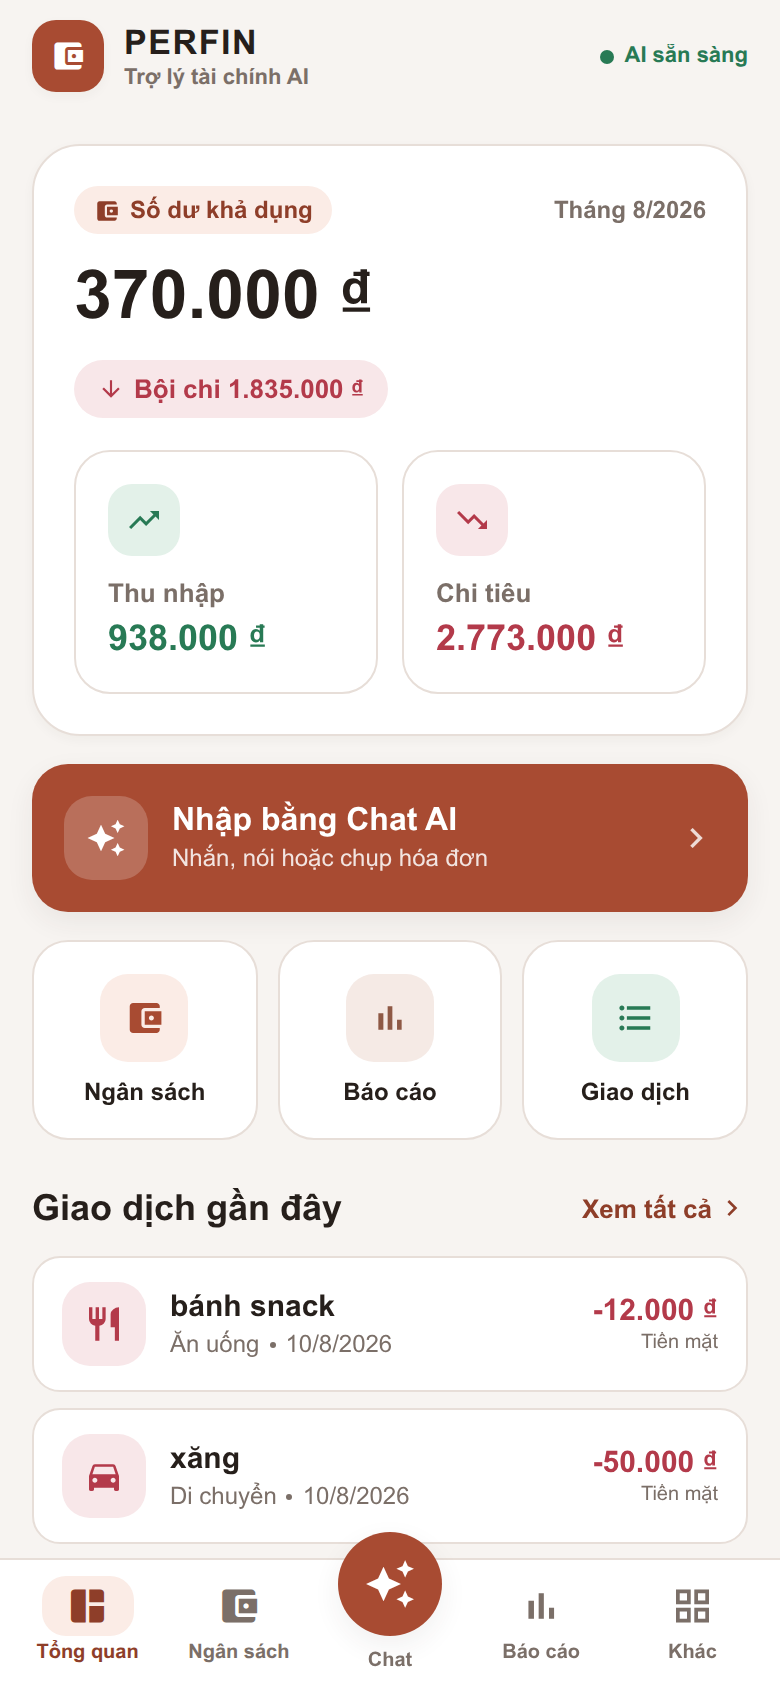
\includegraphics[width=\linewidth,height=0.48\textheight,keepaspectratio]{figures/screenshots/01-dashboard.png}
  \end{minipage}\hfill
  \begin{minipage}[t]{0.47\textwidth}
    \centering
    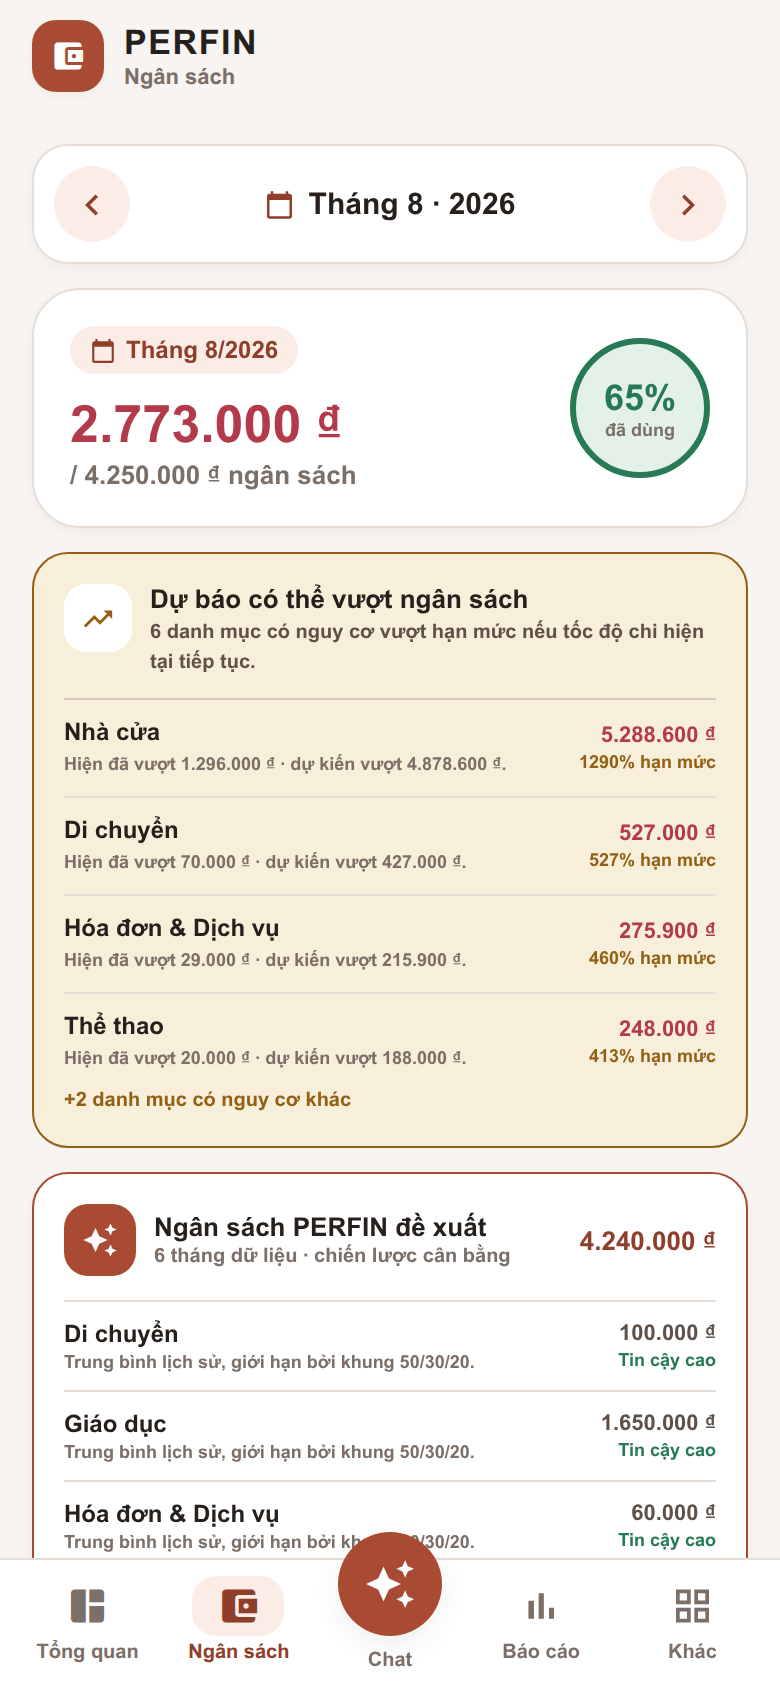
\includegraphics[width=\linewidth,height=0.48\textheight,keepaspectratio]{figures/screenshots/03-budget.png}
  \end{minipage}
  \caption{Smoke Expo web mobile: Dashboard và Budget (dữ liệu synthetic; không phải thiết bị vật lý).}
  \label{fig:ui-dashboard-budget}
\end{figure}

\begin{figure}[p]
  \centering
  \begin{minipage}[t]{0.47\textwidth}
    \centering
    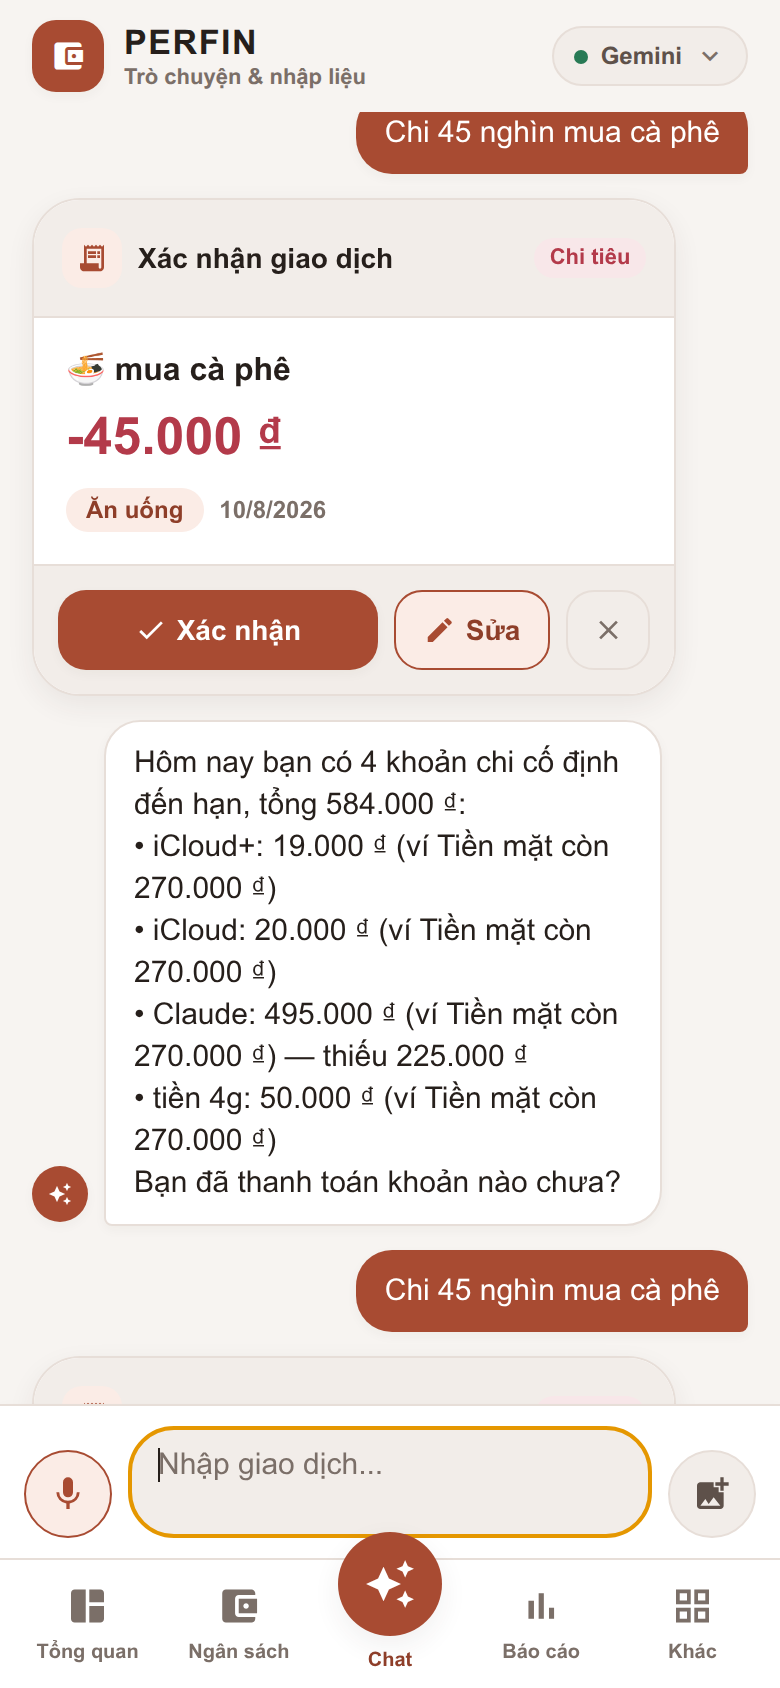
\includegraphics[width=\linewidth,height=0.48\textheight,keepaspectratio]{figures/screenshots/02-chat-preview.png}
  \end{minipage}\hfill
  \begin{minipage}[t]{0.47\textwidth}
    \centering
    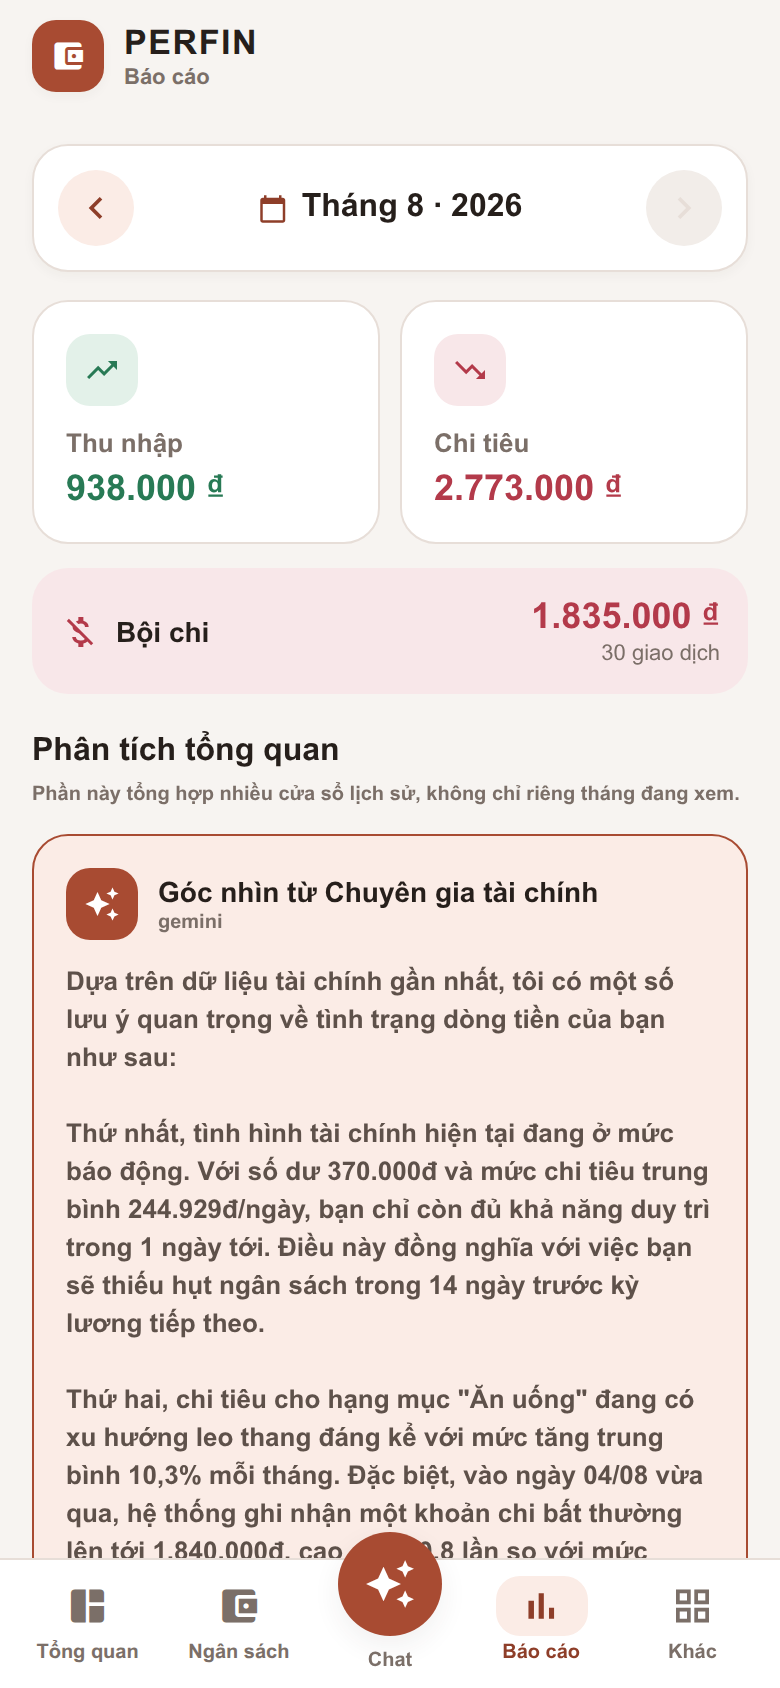
\includegraphics[width=\linewidth,height=0.48\textheight,keepaspectratio]{figures/screenshots/04-report.png}
  \end{minipage}
  \caption{Smoke Expo web mobile: Chat preview trước xác nhận và Report đã tải xong (dữ liệu synthetic; không phải UAT).}
  \label{fig:ui-chat-report}
\end{figure}

\section{Thiết kế phần mềm}

\subsection{Kiến trúc ứng dụng}

PERFIN chọn modular monolith: các route, service, model và engine được tách theo trách nhiệm nhưng API vẫn triển khai trong một tiến trình; worker là tiến trình riêng cho job nền. Cách này phù hợp quy mô niên luận, giảm chi phí vận hành và vẫn cho phép kiểm thử module độc lập.

\widereportfigure{02-runtime-architecture.pdf}{Kiến trúc vận hành của PERFIN; lõi xác định tạo và lưu facts, còn AI Orchestrator chỉ điều phối ngữ nghĩa.}{fig:runtime-architecture}

\begin{table}[H]
  \centering
  \caption{Thành phần kiến trúc và trách nhiệm}
  \label{tab:components}
  \begin{tabularx}{\textwidth}{@{}L{3.2cm}Y Y@{}}
    \toprule
    \textbf{Thành phần} & \textbf{Trách nhiệm} & \textbf{Không chịu trách nhiệm} \\
    \midrule
    Mobile App & Thu input, hiển thị preview/facts và xác nhận. & Truy cập DB hoặc giữ secret AI. \\
    Express Routes & HTTP contract, upload và validation đầu vào. & Chứa công thức phân tích. \\
    Core Services & Luật nghiệp vụ, transaction và idempotency. & Sinh số liệu bằng LLM. \\
    Analytics, Budget, Goal & Tính facts và kế hoạch xác định. & Viết lời khuyên tùy ý. \\
    AI Orchestrator & Tool routing, extraction, narration và fallback. & Ghi DB không qua service. \\
    PostgreSQL & Dữ liệu chuẩn, constraint và truy vấn tổng hợp. & Lưu state hội thoại tạm. \\
    Redis/BullMQ & TTL state, cache, queue và retry. & Làm nguồn sự thật tài chính. \\
    \bottomrule
  \end{tabularx}
\end{table}

Phương án microservice đã được cân nhắc nhưng không chọn vì số module và tải của nguyên mẫu chưa bù được chi phí triển khai, tracing và nhất quán phân tán. Serverless cũng không phù hợp với worker dài hạn và provider media cục bộ. Modular monolith giữ transaction cơ sở dữ liệu đơn giản, đồng thời cho phép tách service về sau nếu có bằng chứng tải thực tế.

\subsection{Thiết kế dữ liệu}

\widereportfigure{04-domain-class.pdf}{Class Diagram UML của miền PERFIN, tách sổ cái, kế hoạch, recurring và hội thoại/phản hồi.}{fig:domain-class}

Hình~\ref{fig:domain-class} mô tả các lớp miền và bội số quan hệ. \code{User} là gốc sở hữu; \code{Wallet}, \code{Transaction} và \code{Category} tạo sổ cái; \code{Budget}, \code{FinancialGoal} và các lớp recurring tạo kế hoạch; \code{ChatMessage} và \code{AIFeedback} lưu tương tác cần truy vết. Các engine không xuất hiện như entity vì chúng chỉ đọc dữ liệu và tạo facts.

\widereportfigure{05-physical-erd.pdf}{ERD vật lý được đối chiếu với chuỗi migration runtime; các khóa ngoại nghiệp vụ chính đi theo những hành lang trực giao tách biệt.}{fig:physical-erd}

\begin{longtable}{@{}L{4.5cm}L{3.0cm}L{6.0cm}@{}}
  \caption{Danh sách thực thể theo thứ tự bảng chữ cái}\label{tab:data-entities}\\
  \toprule
  \textbf{Thực thể} & \textbf{Kiểu} & \textbf{Mô tả} \\
  \midrule
  \endfirsthead
  \toprule
  \textbf{Thực thể} & \textbf{Kiểu} & \textbf{Mô tả} \\
  \midrule
  \endhead
  \code{ai_feedback_logs} & Lịch sử & Kết quả AI ban đầu, correction và ngữ cảnh. \\
  \code{ai_personalities} & Danh mục & Persona và style prompt có thể chọn. \\
  \code{backup_config} & Cấu hình & Chính sách backup theo người dùng; chưa chứng minh worker backup. \\
  \code{budget_history} & Lịch sử & Dấu vết thay đổi hạn mức. \\
  \code{budgets} & Kế hoạch & Hạn mức theo danh mục và tháng. \\
  \code{categories} & Danh mục & Taxonomy thu/chi và quan hệ cha--con. \\
  \code{chat_messages} & Lịch sử & Nội dung hội thoại, facts/metadata và event key. \\
  \code{export_history} & Vận hành & Tệp xuất, bộ lọc và thời điểm hết hạn. \\
  \code{financial_goals} & Kế hoạch & Mục tiêu, tiến độ, hạn chót và ví liên kết. \\
  \code{investment_pnl} & Sổ cái & Lãi/lỗ ghi nhận cho ví đầu tư. \\
  \path{recurring_bill_payments} & Sổ cái & Thanh toán của từng kỳ recurring bill. \\
  \code{recurring_bills} & Kế hoạch & Số tiền, tần suất và ngày đến hạn kế tiếp. \\
  \path{recurring_suggestions_dismissed} & Lịch sử & Chữ ký gợi ý định kỳ đã bị bỏ qua. \\
  \code{transactions} & Sổ cái & Giao dịch thu/chi, nguồn nhập và trạng thái soft delete. \\
  \code{user_traits} & Cá nhân hóa & Trait chỉ dùng khi người dùng đồng ý. \\
  \code{users} & Gốc dữ liệu & Hồ sơ demo và khóa phạm vi dữ liệu. \\
  \code{wallet_transfers} & Sổ cái & Chuyển tiền giữa hai ví. \\
  \code{wallets} & Sổ cái & Số dư, loại và tên ví. \\
  \bottomrule
\end{longtable}

Tiền dùng \code{DECIMAL(15,2)}; truy vấn báo cáo loại bản ghi soft delete; xóa danh mục có giao dịch phải bị chặn hoặc re-tag có kiểm soát; pending/clarification chỉ nằm trong Redis; mọi truy vấn theo ID trong thiết kế đích phải kèm \code{user_id/user_key}. Chuyển nội bộ chỉ nhận hai ví cùng tiền tệ; runway chỉ cộng các ví VND thanh khoản thuộc loại \code{cash}, \code{bank} hoặc \code{e_wallet}. Ngoại tệ, tiết kiệm, đầu tư và thẻ tín dụng bị loại vì nguyên mẫu chưa có tỷ giá hoặc mô hình thanh khoản.

\subsection{Thiết kế chi tiết}
\label{subsec:detailed-design}

\subsubsection{Ranh giới LLM và nhập liệu}

\widereportfigure{06-llm-boundary.pdf}{Ranh giới trách nhiệm của LLM: typed draft và narration nằm ngoài lõi validation, tính toán và ghi dữ liệu.}{fig:llm-boundary}

LLM chỉ tạo lệnh có kiểu hoặc diễn giải facts. Backend kiểm tra schema và luật miền, dựng preview, chờ xác nhận rồi mới mở transaction. Với truy vấn phân tích, SQL và engine tạo facts trước khi narrator được gọi. Khi provider lỗi, parser hoặc template là fallback có thể kiểm thử.

\widereportfigure{08-text-sequence.pdf}{Sơ đồ tuần tự nhập giao dịch bằng văn bản; transaction ghi dữ liệu chỉ bắt đầu sau xác nhận.}{fig:text-sequence}

Hình~\ref{fig:text-sequence} thể hiện hai giai đoạn tách biệt: parse/preview không có side effect và confirm/commit có claim pending. State gồm intent, trường thiếu, candidates và draft, có TTL 5 phút. Xác nhận đồng thời phải dùng claim nguyên tử để một \code{pending_id} không tạo hai giao dịch.

\widereportfigure{09-multimodal-flow.pdf}{Flowchart xử lý ảnh và giọng nói; hai nhánh hội tụ vào pipeline văn bản sau khi raw text được kiểm tra.}{fig:multimodal-flow}

OCR/STT chỉ trả raw text và metadata provider. Phiên bản hiện tại chưa có ground truth đủ lớn và chưa tự đối soát tổng dòng hàng với tổng hóa đơn; vì vậy Hình~\ref{fig:multimodal-flow} là thiết kế luồng, không phải bằng chứng accuracy.

\subsubsection{Phân loại và correction retrieval}
\label{subsec:classification-design}

\widereportfigure{10-feedback-flow.pdf}{Luồng phân loại và correction retrieval; feedback chỉ được ghi sau khi người dùng xác nhận.}{fig:feedback-flow}

Điểm tổng hợp dùng trong matcher là

\begin{equation}
  s=\max(s_{edit},\;0{,}92s_{dice},\;s_{contain}).
\end{equation}

Với $U,V$ là hai tập token sau chuẩn hóa và chọn $|U|\leq|V|$, điểm bao hàm trong mã nguồn được định nghĩa là

\begin{equation}
  s_{contain}=\begin{cases}
    \min\!\left(0{,}94,\;0{,}82+0{,}12\dfrac{|U|}{|V|}\right),
      & U\subseteq V\ \text{và}\ |U|\geq2,\\
    0, & \text{trường hợp khác}.
  \end{cases}
\end{equation}

Thứ tự chọn là exact tên, exact alias rồi fuzzy. Độ dài input được tính sau chuẩn hóa; input trên bốn ký tự dùng ngưỡng $\tau=0{,}82$, input không quá bốn ký tự dùng $\tau=0{,}90$; ứng viên tốt nhất phải hơn ứng viên thứ hai ít nhất $m=0{,}08$. Đây là tham số khởi đầu của nguyên mẫu, chưa phải ngưỡng tối ưu cho mọi người dùng. Correction retrieval nạp tối đa 200 mẫu gần đây và chỉ override bằng bản ghi có cùng loại thu/chi; bản ghi cũ thiếu type không đủ điều kiện. Fuzzy correction cần điểm ít nhất 0,88; khi có nhãn cạnh tranh, nhãn tốt nhất cần agreement ít nhất 0,8. Nhiều nhãn cho cùng exact text trả fallback/làm rõ thay vì bỏ phiếu đa số.

\subsubsection{Giải thuật phân tích và lập kế hoạch}
\label{subsec:analytics-design}

Các cửa sổ mặc định là 14 ngày lịch cho runway, 30 ngày lịch cho anomaly, 200 ngày cho recurring, 6 tháng hoàn tất cho trend, 60 ngày lịch cho phân tích theo thứ và 12 tuần ISO hoàn tất cho correlation. Trục ngày/tháng/tuần cố định được điền 0 ở kỳ không phát sinh. Kỳ tháng/tuần hiện tại còn dở không được đưa vào phép so sánh. Payday là ngày trong tháng theo lịch địa phương; ngày 31 được chặn ở ngày cuối của tháng đích.

Runway chỉ dùng số dư thanh khoản VND:

\begin{equation}
  B=\sum_{\substack{w.currency=\mathrm{VND}\\
  w.type\in\{\mathrm{cash},\mathrm{bank},\mathrm{e\_wallet}\}}} balance_w.
\end{equation}

Với chi ngày $e_j$ và cửa sổ $W=14$, phép tính là

\begin{equation}
  \bar e_W=\frac{1}{W}\sum_{j=1}^{W}e_j,\qquad
  d=\left\lfloor\frac{B}{\bar e_W}\right\rfloor.
\end{equation}

Nếu $B\leq0$ thì $d=0$; nếu $\bar e_W=0$ thì ngày cạn không xác định. Với chuỗi chi tháng $y_j$, trend vẫn giữ trục 6 tháng có zero-fill nhưng cần ít nhất ba tháng quan sát có chi dương; sau đó dùng OLS và chỉ phát tín hiệu khi slope $b>0$, $R^2\geq0{,}5$ và trung bình biến đổi theo bước (chỉ ở bước có mẫu trước dương) ít nhất 10\%.

Anomaly dùng trung bình và độ lệch chuẩn mẫu trên đủ 30 ngày. Chỉ tính anomaly khi có ít nhất bốn ngày lịch có chi dương; quan sát chỉ được gắn cờ ở phía tăng khi

\begin{equation}
  z_i=\frac{e_i-\bar e}{s}\geq2{,}5
  \quad\text{hoặc}\quad
  e_i>Q_3+1{,}5\,IQR.
\end{equation}

Khi $s=0$, mã nguồn đặt $z_i=0$; khi $IQR=0$, nhánh IQR bị tắt. Vì vậy chuỗi hằng không bị gắn cờ chỉ do mẫu số không xác định.

Recurring grouping chuẩn hóa mô tả và cần đồng thời ít nhất ba lần xuất hiện, mọi $\delta_i=|a_i-\bar a|/\bar a\leq0{,}15$, và hệ số biến thiên của khoảng ngày $CV_g=\sigma_g/\bar g\leq0{,}12$ ($\sigma_g$ theo population trên các khoảng dương). Mọi khoảng phải cùng thuộc một cadence: tuần 5--9 ngày, tháng 26--35 ngày hoặc quý 80--100 ngày. Candidate chỉ còn active nếu lần gần nhất không cũ hơn khoảng tối đa của cadence; output ghi thêm \code{lastSeen} và \code{nextExpected} theo lịch có clamp ngày cuối tháng. Không có trần tiền mặc định. Ước tính theo tháng là

\begin{equation}
  \widehat a_{month}=\begin{cases}
    \bar a\,52/12, & \text{tuần},\\
    \bar a, & \text{tháng},\\
    \bar a/3, & \text{quý}.
  \end{cases}
\end{equation}

Correlation điền 0 trên cùng trục 12 tuần, chỉ giữ danh mục có phát sinh ở ít nhất bốn tuần và bỏ cặp Pearson không xác định (ít hơn ba cặp quan sát hoặc một chuỗi không có phương sai). Hệ thống chỉ trả cặp đồng biến mạnh nhất nếu $r\geq0{,}6$; kết quả không hàm ý nhân quả. Phân tích theo thứ dùng cửa sổ 60 ngày, cần ít nhất bốn thứ có dữ liệu và chỉ phát tín hiệu khi tỷ lệ đỉnh so với trung bình đạt 1,8.

Với chi danh mục $s_{c,j}$ trong $m$ tháng, hạn mức nền có buffer 5\% là

\begin{equation}
  b_c=1{,}05\left(\frac{1}{m}\sum_{j=1}^{m}s_{c,j}\right).
\end{equation}

Forecast cuối tháng dùng $\widehat S_D=(S/d_e)D$, trong đó $S$ là số đã chi, $d_e$ là số ngày lịch đã trôi qua tính cả ngày hiện tại và $D$ là số ngày trong tháng. Chiến lược 50/30/20 và hybrid co tỷ trọng khi tổng hạn mức thô vượt trần; bước đối soát sau làm tròn bảo đảm tổng từng nhóm không vượt trần. Các tỷ lệ nhu cầu, mong muốn và tiết kiệm không được có tổng lớn hơn 1; mọi đề xuất cần xác nhận.

Với mục tiêu saving/purchase còn thiếu $R$ và mức góp tháng $M>0$, số tháng là $n_s=\lceil R/M\rceil$. Với khoản nợ hiện còn $L$, lãi suất năm danh nghĩa $i$ tính theo phần trăm, mã nguồn dùng lãi suất tháng $r=i/(12\times100)$. Nếu có hạn nợ trong $n_d$ tháng, mức trả đều cuối tháng cần thiết là

\begin{equation}
  P=\frac{Lr}{1-(1+r)^{-n_d}}
\end{equation}

khi $r>0$; nếu $r=0$ thì $P=L/n_d$. Payment nhỏ hơn hoặc bằng lãi tháng đầu tạo cảnh báo negative amortization; payment bằng 0 được báo riêng. Không có deadline, mã nguồn mô phỏng từng tháng tối đa 600 tháng. What-if hiện chỉ chạy lại hàm saving/purchase với khoản góp thêm; không thay đổi kế hoạch debt và không ghi dữ liệu.

\widereportfigure{12-goal-flow.pdf}{Flowchart lập kế hoạch mục tiêu và what-if; chỉ bước xác nhận cuối cùng mới lưu dữ liệu.}{fig:goal-flow}

\subsubsection{Sinh insight có căn cứ}

\widereportfigure{11-insight-sequence.pdf}{Sơ đồ tuần tự sinh insight; Analytics Engine trả facts trước khi persona/LLM diễn giải.}{fig:insight-sequence}

Contract facts phiên bản 1.0 trả \code{schema_version}, \code{generated_at}, value của từng component và \code{metadata.components}. Metadata mỗi component có \code{unit}, \code{window}, \code{sample_count}, \code{method}, \code{parameters}, \code{warnings} và \code{status} thuộc \code{ok/no_signal/degraded}. Object window ghi \code{size}, \code{unit} và \code{zero_filled}; một số component thêm \code{category_count} hoặc \code{wallet_count}. Lỗi cục bộ được ghi trong \code{degraded_components} mà không làm mất contract. Persona chỉ thay giọng điệu khi consent bật; response trả narration cùng facts để UI/test đối chiếu. Numeric checker bao phủ mọi biểu thức số vẫn là thiết kế đích.

Quy trình tính, ví dụ số và các trường hợp biên của matcher, correction, Analytics, Budget, Goal và facts contract được mở rộng tại Phụ lục~\ref{app:algorithms}--\ref{app:facts-contract}; Chương này giữ các công thức và quyết định thiết kế chính để bảo đảm mạch trình bày.

\section{Kiểm thử}
\label{sec:testing}

\subsection{Kế hoạch kiểm thử}

\begin{longtable}{@{}L{2.2cm}L{3.7cm}L{4.2cm}L{3.9cm}@{}}
  \caption{Ma trận kế hoạch kiểm thử}\label{tab:test-matrix}\\
  \toprule
  \textbf{Cấp} & \textbf{Đối tượng} & \textbf{Kỹ thuật} & \textbf{Bằng chứng dự kiến} \\
  \midrule
  \endfirsthead
  \toprule
  \textbf{Cấp} & \textbf{Đối tượng} & \textbf{Kỹ thuật} & \textbf{Bằng chứng dự kiến} \\
  \midrule
  \endhead
  Unit & Matching, analytics, budget, goal, validation. & Ca thường, biên, expected tính tay và invariant. & \code{node:test}, pass/fail từng ca. \\
  Integration & Route--service--model, PostgreSQL, Redis. & DB test, rollback, TTL và claim đồng thời. & Log, snapshot DB và mã thoát. \\
  System & Text/voice/image đến preview/DB. & Smoke theo kịch bản end-to-end. & HTTP response, DB assertion, ảnh UI. \\
  AI contract & Parser, tool schema, LLM và correction. & Nhãn joint type/category; abstention giữ trong mẫu số; split nguyên nhóm. & JSON records, coverage, accuracy/F1, helped/harmed/net. \\
  Media & OCR/STT adapter. & Ảnh/audio có ground truth. & CER/WER và field accuracy. \\
  Worker & Retry, dedup và lịch chạy. & Lặp cùng fingerprint, fault injection. & Số hiệu ứng trước--sau. \\
  UAT & Người dùng mục tiêu. & Nhiệm vụ có thời gian và số bước. & Completion rate, thời gian, SUS. \\
  \bottomrule
\end{longtable}

Bộ dữ liệu văn bản cần bao phủ đơn vị tiền, số bằng chữ, phép nhân, ngày tương đối, nhiều giao dịch, typo, Việt--Anh, trường hợp thiếu/mơ hồ và correction xung đột. Khi đánh giá correction, mọi dòng cùng loại và mô tả chuẩn hóa phải nằm hoàn toàn ở seed hoặc evaluation. Dữ liệu analytics dùng chuỗi tổng hợp hoặc ẩn danh có slope, outlier, cadence và correlation biết trước. Tập media phải lưu ảnh/audio cùng transcript hoặc bảng hóa đơn chuẩn.

Danh mục ca thường, ca biên, invariant và tệp kiểm thử tương ứng được lập thành ma trận ở Phụ lục~\ref{app:algorithm-tests}; mô tả nguồn, schema, cohort và giới hạn của dataset nằm ở Phụ lục~\ref{app:dataset-description}. Các bảng phụ lục chỉ dẫn đến bằng chứng và không thay thế các kết quả đã công bố trong mục~\ref{subsec:results}.

\subsection{Kết quả và phân tích}
\label{subsec:results}

\subsubsection{Kết quả vận hành đã đo}

\begin{longtable}{@{}L{3.4cm}L{3.5cm}L{2.4cm}L{4.4cm}@{}}
  \caption{Kết quả đo và giới hạn kết luận}\label{tab:measured-results}\\
  \toprule
  \textbf{Hạng mục} & \textbf{Kết quả} & \textbf{Trạng thái} & \textbf{Phạm vi kết luận} \\
  \midrule
  \endfirsthead
  \toprule
  \textbf{Hạng mục} & \textbf{Kết quả} & \textbf{Trạng thái} & \textbf{Phạm vi kết luận} \\
  \midrule
  \endhead
  Regression mục tiêu (21 ca) & 21/21 đạt cho analytics, invariant và ranh giới provider media. & \statusmeasured & Lệnh và fixture có thể tái lập; đây là tập con tập trung, không phải full suite. \\
  Backend \code{npm test} & 247/247 test đạt khi tắt Redis và jobs. & \statusmeasured & Full suite đạt trên worktree hiện tại; chưa đo hành vi Redis worker live. \\
  Coverage Node 24 & 68,12\% line, 72,77\% branch và 72,27\% function trên toàn bộ file backend đã load. & \statusmeasured & Lệnh có thể tái lập; các ngưỡng mục tiêu theo component (line/function $\geq85\%$, branch $\geq75\%$) chưa được chứng minh. \\
  Local-parser gate và API smoke & Chờ chạy sạch trên snapshot hiện tại. & \statusmissing & Artifact trước thuộc worktree cũ và không còn là bằng chứng hiện tại. \\
  Mobile-web UI smoke & 5/5 capture synthetic đạt ở 390$\times$844. & \statusmeasured & Dashboard, Budget, Report, Chat preview và Goal plan tải xong, không overflow; chỉ là Expo web, không phải native-device hay UAT. \\
  Data profile & 5.328 dòng nguồn, 0 lỗi validation; SHA prefix \code{418a...}. & \statusmeasured & Dry-run bao phủ 01/01/2022--10/08/2026; apply vào PostgreSQL là bước riêng. \\
  Current experiments & Chờ rerun trên snapshot 5.328 dòng. & \statusmissing & Metric chính là joint type/category; correction phải mô phỏng candidate limit 200 của production. \\
  Ablation parser--Gemini & Chờ chạy lại với joint label và record đầy đủ theo mẫu. & \statusmissing & Category-only chỉ là phụ; abstention vẫn nằm trong mẫu số. \\
  Accuracy OCR/STT & Chờ ground truth 20 ảnh và 20 audio. & \statusmissing & Không thể suy ra CER/WER hay field accuracy từ smoke execution. \\
  Redis worker live, grounding, p95 và UAT & Chờ môi trường có kiểm soát và người tham gia mục tiêu. & \statusmissing & Cần assert duplicate-effect, checker, ít nhất 30 lượt/luồng và từ năm người dùng. \\
  \bottomrule
\end{longtable}

Smoke test chỉ chứng minh khả năng hoàn tất kịch bản đã chọn. Vì chưa có ground truth media, báo cáo không gọi OCR/STT là ``đã đo độ chính xác''. Tương tự, việc logic payment/handler vượt qua unit test không đồng nghĩa Redis worker đã chạy live.

\subsubsection{Thí nghiệm phân loại}

Nguồn hiện tại là \code{demo/data/dataFinance.csv}, được profile ở 5.328 dòng với tiền tố SHA-256 \code{418a9439...fbaed7}. Các artifact classification, ablation và correction dùng file 5.265 dòng trước đây vẫn giữ để audit nhưng đã superseded, không được báo như kết quả hiện tại.

Quy trình rerun được khóa trước khi nhận data mới:

\begin{table}[H]
  \centering
  \caption{Quy trình rerun classification và correction}
  \label{tab:exp-classification}
  \begin{tabularx}{\textwidth}{@{}L{3.0cm}Y Y@{}}
    \toprule
    \textbf{Thí nghiệm} & \textbf{Đo lường chính} & \textbf{Bằng chứng bắt buộc} \\
    \midrule
    Local parser & Accuracy, macro-F1, weighted-F1 và support theo lớp trên nhãn joint type/category; category-only là phụ. & Hash CSV hiện tại, prediction đầy đủ theo dòng và lệnh deterministic. \\
    Parser--Gemini ablation & Coverage joint-label, accuracy/F1 toàn mẫu, metric trên câu trả lời và latency; abstention vẫn trong mẫu số. & Record từng mẫu, model/cấu hình và số lỗi provider. \\
    Correction retrieval & Nhãn joint trước/sau, coverage và helped/harmed/net dưới group split theo thời gian. & Candidate limit 200, không dùng dòng tương lai, overlap khóa seed/evaluation bằng 0 và khoảng tin cậy. \\
    \bottomrule
  \end{tabularx}
\end{table}

Runner correction hiện ghi candidate limit production-equivalent là 200 và số candidate theo từng dòng. Thứ tự hiện dùng source-row như proxy thời gian có ghi rõ; khi có timestamp đáng tin, cần thay bằng temporal replay thực. Runner ablation hiện đặt nhãn joint type/category làm metric chính, còn category-only chỉ là góc nhìn phụ.

\begin{table}[H]
  \centering
  \caption{Trạng thái artifact thí nghiệm trên snapshot hiện tại}
  \label{tab:exp-ablation}
  \begin{tabularx}{\textwidth}{@{}L{4.0cm}L{3.0cm}Y@{}}
    \toprule
    \textbf{Artifact} & \textbf{Trạng thái} & \textbf{Lý do chưa đưa điểm số} \\
    \midrule
    Local classification & \statusmissing & Artifact cũ dùng CSV khác và phải sinh lại. \\
    Parser--Gemini ablation & \statusmissing & Record cũ thiếu prediction joint đầy đủ; rerun cần provider/quota. \\
    Correction retrieval & \statusmissing & Runner cũ đưa toàn bộ seed log thay vì cửa sổ 200 candidate như production. \\
    \bottomrule
  \end{tabularx}
\end{table}

Các trạng thái này giữ truy vết mà không biến thí nghiệm lịch sử thành claim về mã nguồn hoặc dataset hiện tại. Khi bạn cung cấp fixture có kiểm soát, JSON và Markdown mới có thể chèn vào mà không đổi định nghĩa metric.

\subsection{Truy vết yêu cầu và bằng chứng}

Ma trận truy vết ở Bảng~\ref{tab:traceability} liên kết mục tiêu quan sát được với thiết kế, kiểm thử và trạng thái bằng chứng. Một chức năng chỉ được xem là đã chứng minh trong phạm vi cột cuối; việc có route, mock hoặc sơ đồ không tự động đồng nghĩa đã nghiệm thu end-to-end.

\begin{longtable}{@{}L{2.2cm}L{3.4cm}L{3.5cm}L{4.8cm}@{}}
  \caption{Ma trận truy vết FR--thiết kế--kiểm thử--bằng chứng}\label{tab:traceability}\\
  \toprule
  \textbf{Yêu cầu} & \textbf{Thiết kế chính} & \textbf{Kiểm thử liên quan} & \textbf{Bằng chứng và khoảng trống} \\
  \midrule
  \endfirsthead
  \toprule
  \textbf{Yêu cầu} & \textbf{Thiết kế chính} & \textbf{Kiểm thử liên quan} & \textbf{Bằng chứng và khoảng trống} \\
  \midrule
  \endhead
  FR-01, FR-03--FR-05 & Typed draft, preview có TTL, service và SQL transaction. & Parser gate; backend unit/service; API--DB smoke. & Có bằng chứng cho fixture chọn trước và invariant rollback; chưa đo thao tác người dùng độc lập. FR-06 được đặc tả ở phụ lục. \\
  FR-02 & Media adapter, raw-text review và pipeline FR-01 dùng chung. & Upload/media smoke; kế hoạch CER, WER và field accuracy. & Đã chứng minh luồng mẫu đi qua provider; chưa đủ ground truth để công bố accuracy OCR/STT. \\
  FR-04 & Joint classifier, correction theo type, ngưỡng conflict và group split. & Benchmark classification; ablation coverage; correction helped/harmed/net. & Chờ rerun trên CSV hiện tại và cửa sổ candidate production; điểm lịch sử đã superseded. \\
  FR-07--FR-10 & Analytics Engine, facts contract, Budget/Goal service và narrator có căn cứ. & Unit với expected tính tay; contract metadata; numeric checker dự kiến. & Công thức, kỳ lịch và metadata có test; grounding toàn bộ response và hiệu chỉnh ngưỡng trên dữ liệu đại diện chưa hoàn tất. \\
  FR-11 & Recurring service, BullMQ, event key và retry. & Unit payment/handler; fault injection và live worker dự kiến. & Logic nghiệp vụ có test nhưng chưa có bằng chứng queue/worker chạy live trong đợt đánh giá. \\
  FR-12 & CSV exporter, export history và TTL cleanup. & Unit escaping; API smoke; kiểm tra file hết hạn dự kiến. & CSV có bằng chứng; nhánh từng gọi là PDF thực chất mới tạo HTML và không được công bố là PDF. \\
  NFR-01--NFR-08 & Constraint, user scope, fallback, idempotency và facts metadata. & Rollback, cross-scope, load, recovery, worker, UAT. & Toàn vẹn trong test đã có bằng chứng; recovery ba giờ, p95, UAT, worker live và numeric faithfulness vẫn là mục tiêu. \\
  \bottomrule
\end{longtable}

\subsection{Đe dọa đến tính hợp lệ}

\subsubsection{Tính hợp lệ nội tại}

Các benchmark phụ thuộc nhãn lịch sử; cùng một mô tả có thể mang nhiều category. Correction mới tách nguyên nhóm theo type+mô tả chuẩn hóa và có overlap bằng 0, nhưng seed/evaluation vẫn đến từ cùng một dataset, chỉ dùng một seed và không có khoảng tin cậy. Mẫu ablation 63 câu nhỏ; hơn nữa artifact lịch sử không lưu đủ prediction và đã tính metric có điều kiện sau khi loại 21 abstention, nên macro-F1 toàn mẫu Gemini không thể khôi phục. Provider cũng biến đổi theo phiên bản/thời điểm; runner mới vì vậy lưu model, tham số, timestamp và records có cấu trúc đã loại trường nhạy cảm.

\subsubsection{Tính hợp lệ cấu trúc}

Quality gate 31/31 đo việc vượt qua các câu được thiết kế, không đo xác suất đúng ngoài mẫu. Smoke test đo khả năng hoàn tất kịch bản, không đo accuracy hoặc mức dễ dùng. Accuracy có thể che khuất lớp hiếm; abstention còn có thể làm metric có điều kiện trông cao hơn. Vì vậy báo cáo kèm coverage, macro-F1, weighted-F1, confusion theo lớp, helped/harmed/net và số mẫu. Với OCR/STT, chỉ CER/WER cũng chưa đủ: field accuracy của amount, date và merchant mới gắn trực tiếp với rủi ro sổ cái.

\subsubsection{Tính hợp lệ ngoại suy}

Dữ liệu thuộc một hồ sơ demo, tiền VND và ngôn ngữ chủ yếu là tiếng Việt; kết quả không tự suy rộng sang nhiều người dùng, taxonomy khác, ảnh hóa đơn đa dạng hoặc môi trường tải production. Vòng đánh giá kế tiếp cần khóa taxonomy, lấy mẫu ngẫu nhiên theo thời gian, giữ group split hiện có nhưng chạy nhiều seed/khoảng tin cậy, và bổ sung người dùng mục tiêu cho UAT. Kết luận chỉ áp dụng cho mã nguồn, dataset và môi trường ghi trong artifact ablation 24/07 cùng classification/correction 02/08/2026.
